% === Begin Label Data ===
% ID: 712
% 难度星级: 
% 标签: 
% 备注: 
% 组卷引用次数: 0
% === End  Label Data ===

\begin{problem}{2011}{G}{湖北卷（理）}{7}{概率}
如图，用 $K$、$A_1$、$A_2$ 三类不同的元件连接成一个系统。当 $K$ 正常工作且 $A_1$、$A_2$ 至少有一个正常工作时，系统正常工作。已知 $K$、$A_1$、$A_2$ 正常工作的概率依次为 $0.9$、$0.8$、$0.8$，则系统正常工作的概率为 \hspace{1cm}（　　）

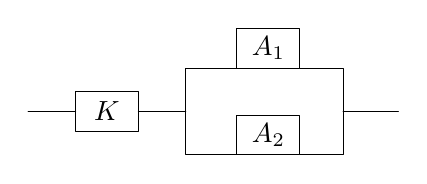
\begin{tikzpicture}[line cap=round,line join=round,scale=1]
\usetikzlibrary{calc}

\draw (-1.2,0) -- (-0.6,0);

\draw (-0.6,-0.25) rectangle (0.2,0.25);
\node at (-0.2,0) {$K$};

\draw (0.2,0) -- (0.8,0);

% parallel branches frame
\coordinate (L) at (0.8,0);
\coordinate (R) at (2.8,0);

\draw (L) -- ++(0,0.55) -- ++(0.4,0) coordinate (Lt);
\draw (L) -- ++(0,-0.55) -- ++(0.4,0) coordinate (Lb);

\draw (R) -- ++(0,0.55) -- ++(-0.4,0) coordinate (Rt);
\draw (R) -- ++(0,-0.55) -- ++(-0.4,0) coordinate (Rb);

% top element A1
\draw (Lt) -- ++(0.25,0) rectangle ++(0.8,0.5);
\node at ($(Lt)+(0.65,0.25)$) {$A_1$};
\draw ($(Lt)+(1.05,0)$) -- (Rt);

% bottom element A2
\draw (Lb) -- ++(0.25,0) rectangle ++(0.8,0.5);
\node at ($(Lb)+(0.65,0.25)$) {$A_2$};
\draw ($(Lb)+(1.05,0)$) -- (Rb);

% right output
\draw (2.8,0) -- (3.5,0);

\end{tikzpicture}
\begin{choices}
\choice{{$0.960$}}
\choice{{$0.864$}}
\choice{{$0.720$}}
\choice{{$0.576$}}
\end{choices}
\end{problem}

\begin{answer}

\end{answer}

\begin{solutions}

\end{solutions}